\section{Introduction}
\label{sec:MissionSites:Introduction}
Mission sites were required before determining environmental constraints pertaining to available solar radiation. Western Iani Chaos and Ismenius Cavus were selected based on the following criteria:

\begin{itemize}
    \item Location is of scientific interest.
    \item Landing sites have been proposed.
    \item Presence of sloped and/or ridged terrain to simulate inclined surface mission scenarios.
    \item Availability of HiRISE digital terrain models (DTM) near the ROI to load 3D environment model in simulation platform.
    \item Planetary latitude proximity to the MER Opportuniy missions in order to enable comparative analysis with 14 years worth of power budget data. The target planetary latitude is approximately \SI{-2}{\degree}.
    \item Planetary latitude proximity to VL1 and VL2 missions in order to more closely align with the environment conditions from which the power and energy prediction models were built. The target planetary latitude is between \SI{22}{\degree} and \SI{48}{\degree}.
\end{itemize}

\subsection{Western Iani Chaos}
\label{sec:MissionSites:WesternIaniChaos}

\subsection{Ismenius Cavus}
\label{sec:MissionSites:IsmeniusCavus}
Ismenius Cavus is at \SI{33.5}{\degree} N, \SI{17}{\degree} E, with elevations ranging from \SI{-3.5}{\kilo\meter}. It is a base where seveal fluvial valleys converge and is located ``at the junction between current mid-latitude ice deposits and low latitude clay minerals'', hosting science and resource regions of interest ``with both present ice and past lake sediments with clay minerals'' \citeother{Dehouck2010} \citeother{Dehouck2015}.

\begin{figure}[h]
  \centering
  \hypersetup{linkcolor=captionTextColor}
  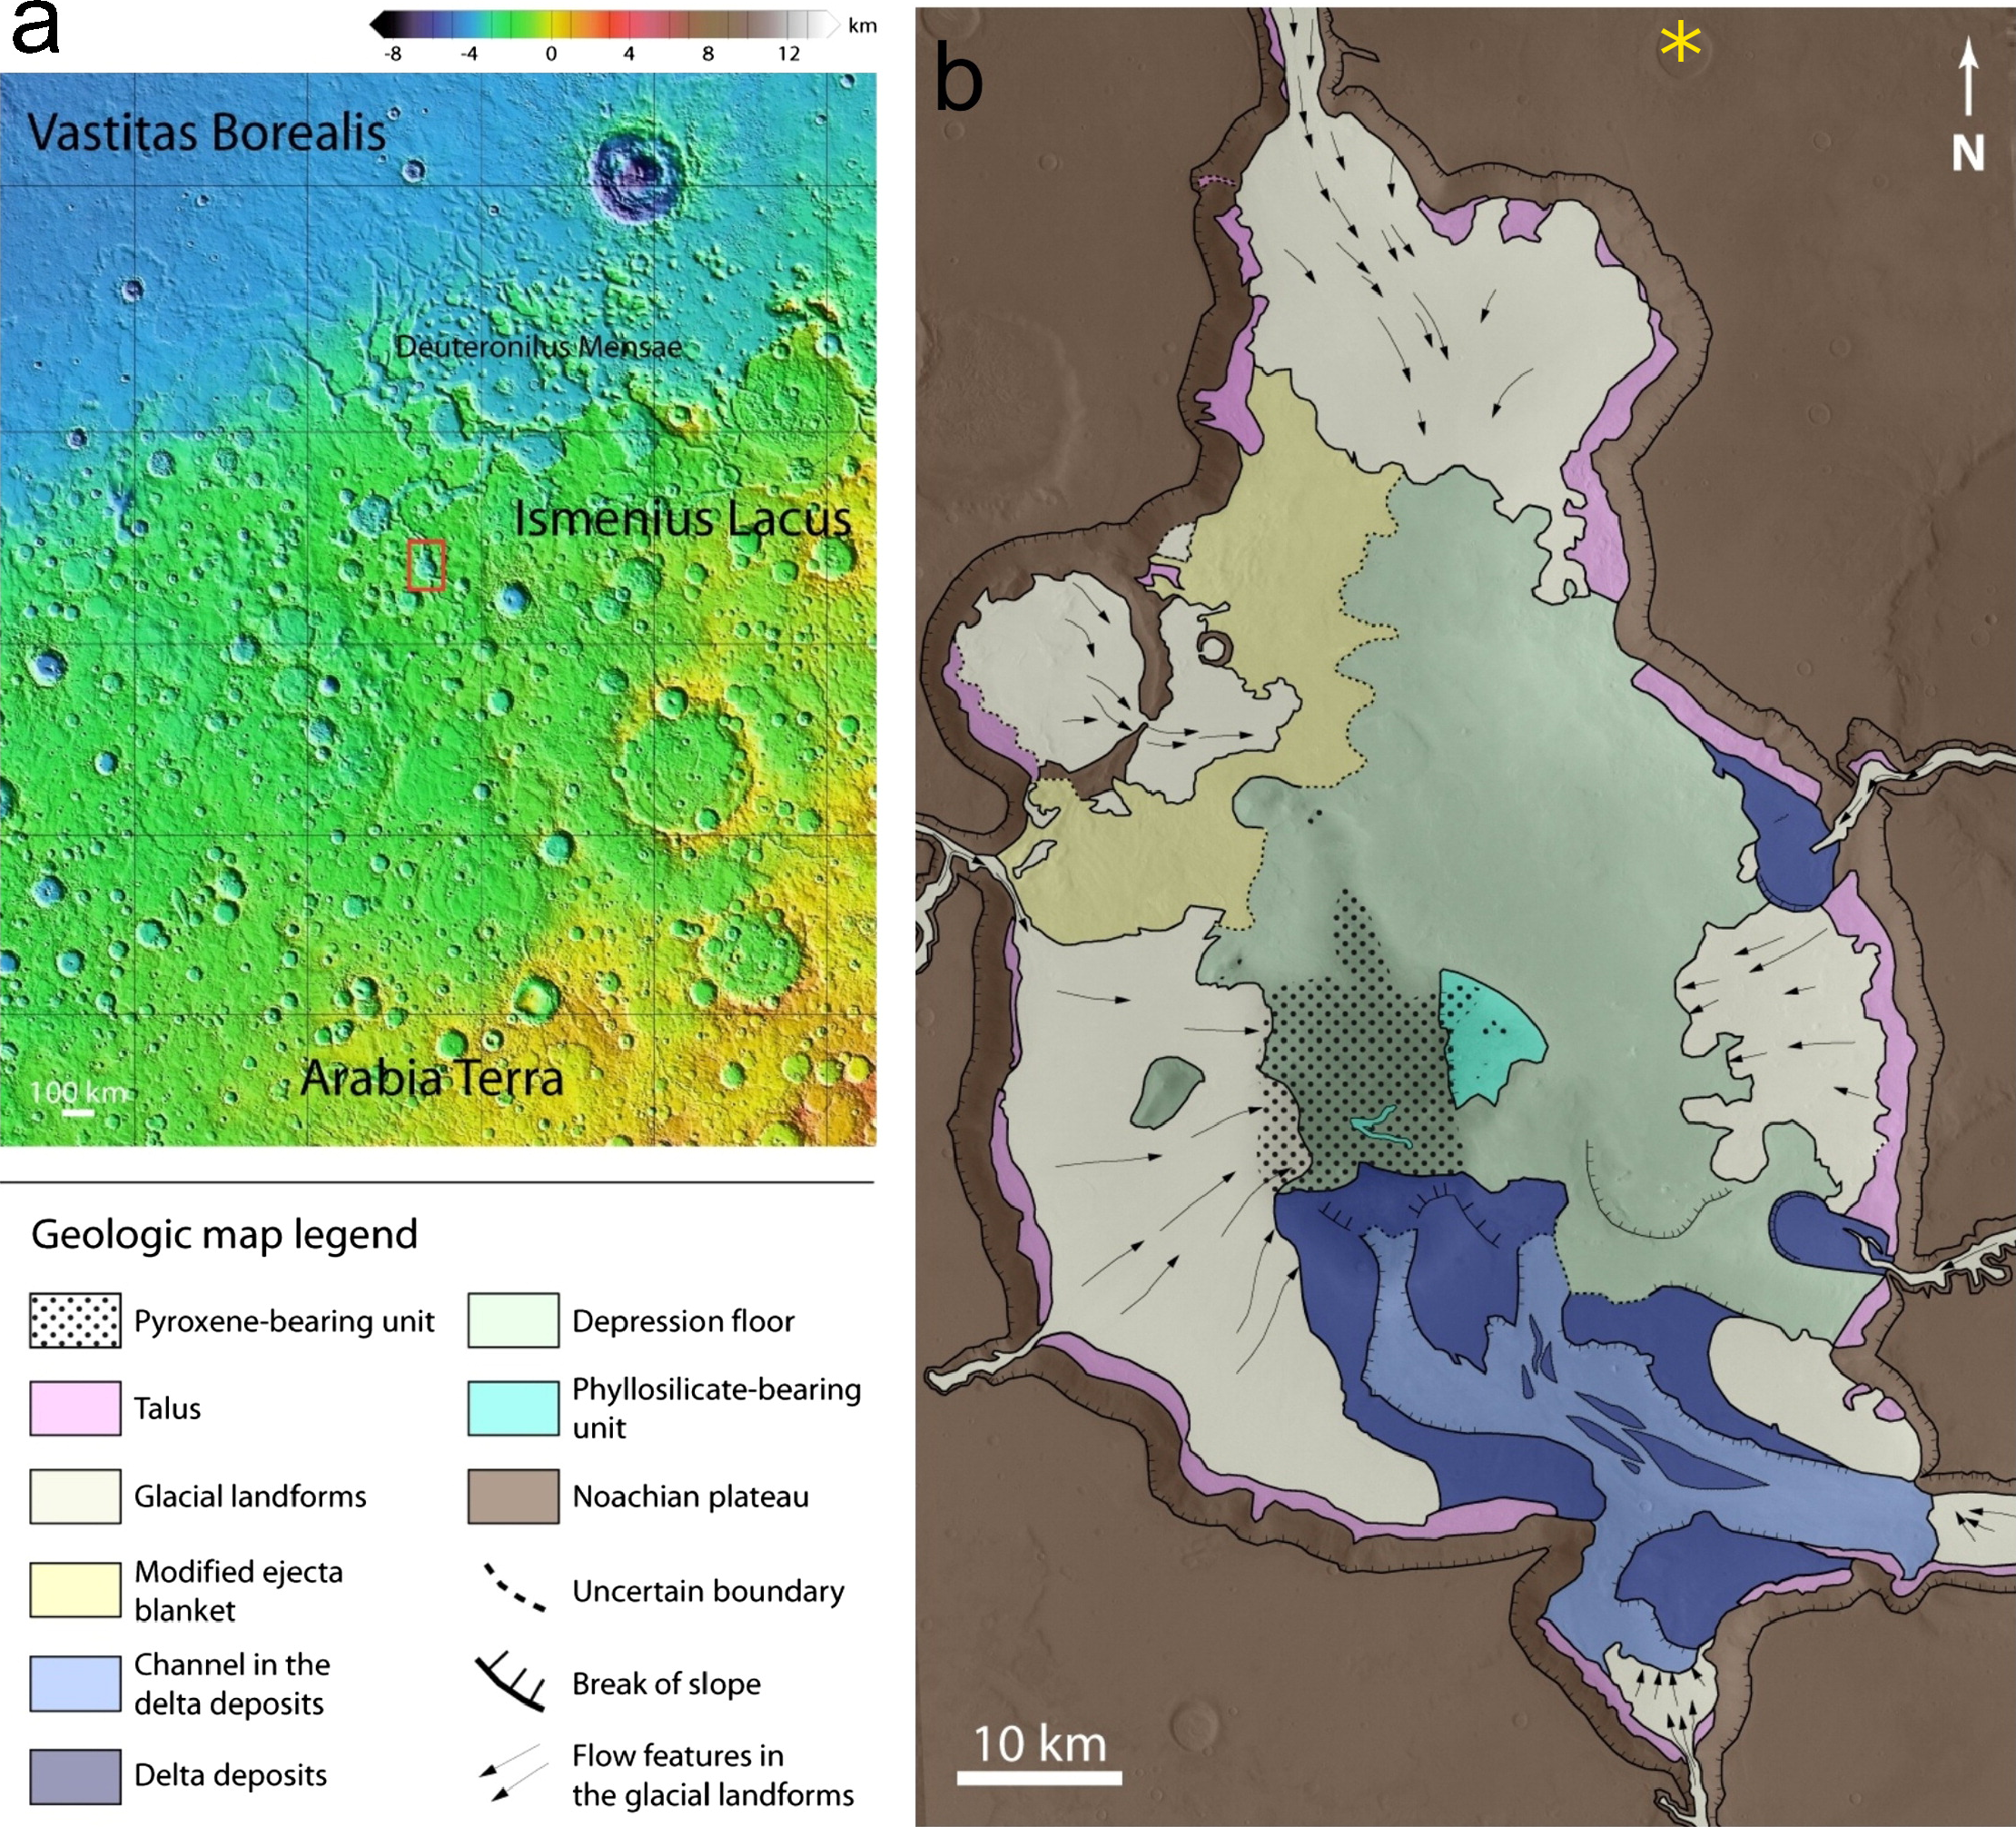
\includegraphics[width=0.8\linewidth]{sections/mission-sites/images/ismenius-cavus.png}\\
  \caption[Geologic context for Ismenius Cavus mission site area]
          {Geologic context of the mission site area, taken from \citeother{Dehouck2010}. Location shown on a MOLA reference map (a) and a geologic map of Ismenius Cavus (b). The yellow asterisk indicates the DTM location used for mission scenario simulation.}
  \label{fig:mission-site-ismenius-cavus}
\end{figure}

% https://www.uahirise.org/dtm/dtm.php?ID=ESP_052945_2150

Supported science of interest are taken from \citeother{Dehouck2015}:
\begin{itemize}
    \item Potential fo past habitability.
    \item Potential for organic matter with surface exposure.
    \item Noachian/Hesperian rocks w/ trapped atmospheric gases.
    \item High likelohood of surface-atmosphere exchange.
    \item Amazonian subsurface or high-latitude ice or sediment.
    \item Range of martian geologic time; datable surfaces.
    \item Evidence of aqueous processes.
    \item Potential for interpreting relative ages.
    \item Near-surface ice, glacial or permafrost.
    \item Noachian or pre-Noachian bedrock units.
    \item Diversity of aeolian sediments and/or landforms.
\end{itemize}

Supported resources of interest are also presented in \citeother{Dehouck2015}, emphasizing two main resources for water with clay minerals and water ice as well as a potential for metal/silicon resources. These are located no more than 3 meters below the surface and can be minable by automated systems. Mobile material resources for construction purposes also exist.

\section{Conclusion}
